\documentclass[11pt,a4paper]{article}
\usepackage[T1]{fontenc}
\usepackage[utf8]{inputenc}
\usepackage{lmodern}
\usepackage{textcomp}
\usepackage[left=1.8cm,right=1.8cm,top=2.3cm,bottom=2.2cm,headheight=14pt,headsep=8pt]{geometry}
\usepackage{multicol}
\usepackage{xcolor}
\usepackage{fancyhdr}
\usepackage{graphicx}
\usepackage{array}
\usepackage{amsmath,amssymb}
\usepackage{setspace}
\usepackage{longtable}
\graphicspath{{../}}
\definecolor{ygreen}{RGB}{46,139,87}
\renewcommand{\normalsize}{\fontsize{10.9}{13.4}\selectfont}
\renewcommand{\familydefault}{\rmdefault}
\setlength{\parindent}{0pt}
\setlength{\columnsep}{0.8cm}
\setlength{\columnseprule}{0.4pt}
\setlength{\multicolsep}{3pt plus 1pt minus 1pt}
\renewcommand{\textsubscript}[1]{\ensuremath{_{\text{\fontsize{8}{8}\selectfont #1}}}}
\renewcommand{\textsuperscript}[1]{\ensuremath{^{\text{\fontsize{8}{8}\selectfont #1}}}}
\newcommand{\qn}[1]{\textbf{\fontsize{11.5}{13}\selectfont #1}}
\newcommand{\qsep}{\par\vspace{1pt}\noindent\rule{0pt}{0.4pt}\par\vspace{5pt}}
\newcommand{\fwrule}{\par\vspace{5pt}\noindent\rule{\linewidth}{1.4pt}\par\vspace{7pt}}
\newsavebox{\fitb}
\newcommand{\fitbox}[1]{\sbox{\fitb}{#1}\ifdim\wd\fitb>\linewidth\resizebox{\linewidth}{!}{\usebox{\fitb}}\else\usebox{\fitb}\fi}
\newcommand{\diqqat}[1]{\par\smallskip\noindent\textbf{Diqqat!} #1\par\medskip}
\newcommand{\javob}{\par\smallskip\noindent\textbf{Javob:} \rule[-2pt]{7.5cm}{0.4pt}\par\smallskip\noindent\textbf{Diqqat!} Javobingizni javoblar varaqasiga ko`chirib yozing.\par\medskip}
\pagestyle{fancy}
\fancyhf{}
\renewcommand{\headrulewidth}{0.4pt}
\fancyhead[L]{\textit{Milliy sertifikat 2026. Kimyo}}
\fancyhead[R]{2-variant}
\fancyfoot[L]{\fontsize{8}{9}\selectfont \textcopyright{} Colba maktabi, 2026}
\fancyfoot[C]{\thepage}
\fancypagestyle{first}{\fancyhf{}\renewcommand{\headrulewidth}{0pt}\fancyfoot[L]{\fontsize{8}{9}\selectfont \textcopyright{} Colba maktabi, 2026}\fancyfoot[C]{\thepage}}
\begin{document}
\normalsize
\thispagestyle{first}
\noindent\fcolorbox{ygreen}{white}{\parbox{\dimexpr\linewidth-2\fboxsep-2\fboxrule\relax}{%
\textbf{\fontsize{13}{15}\selectfont Nazorat testi}\ \textit{\fontsize{10}{12}\selectfont $\cdot$ Aralash test $\cdot$ 2-variant}\hfill
\begin{tabular}[t]{@{}r@{}}\textit{Milliy sertifikat 2026. Kimyo}\\ \textbf{\textit{\fontsize{8}{9}\selectfont Vaqt:}} \textit{\fontsize{10}{12}\selectfont 180 daqiqa}\end{tabular}}}
\par\medskip
\noindent\textit{Davriy jadvaldan foydalanish mumkin.}
\par\medskip
\begin{multicols}{2}
\noindent\qn{1.} Jadvalda ikki tuz eritmasi haqida ma'lumot berilgan:
\begin{center}
\renewcommand{\arraystretch}{1.15}
\fitbox{\begin{tabular}{|c|c|c|}\hline
\textbf{Eritma} & \textbf{Massasi, g} & \textbf{Massa ulushi, \%} \\ \hline
1 & 100 & 20 \\ \hline
2 & 200 & 30 \\ \hline
\end{tabular}}
\end{center}
Eritmalar aralashtirilganda hosil bo`lgan eritmaning massa \textbf{ulushini (\%) aniqlang.}

\noindent A)~\textsl{26,67} \hfill B)~\textsl{25} \hfill C)~\textsl{50} \hfill D)~\textsl{23,33}\par
\qsep
\noindent\qn{2.} CuSO\textsubscript{4}$\cdot$5H\textsubscript{2}O kristallogidratida kristallizatsion suvning massa \textbf{ulushini (\%) aniqlang.}

\noindent A)~\textsl{64} \hfill B)~\textsl{36} \hfill C)~\textsl{18} \hfill D)~\textsl{56,2}\par
\qsep
\noindent\qn{3.} 2-davr elementlari atom radiuslarining o`zgarishi diagrammada ko`rsatilgan.
\begin{center}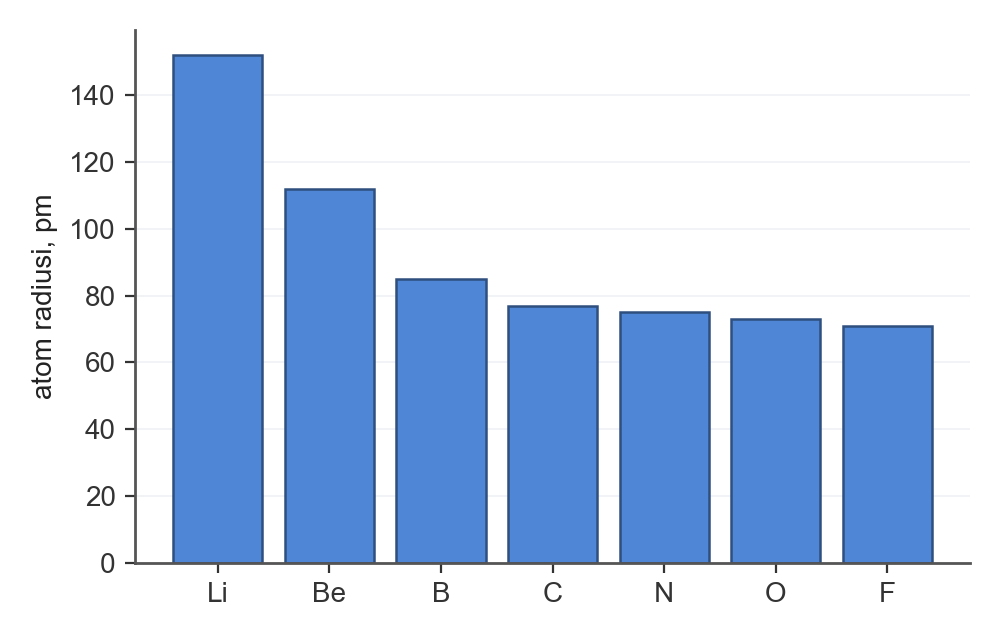
\includegraphics[width=0.86\linewidth]{rasmlar/gen/ra_v02_0.png}\end{center}
Davr bo`yicha chapdan o`ngga atom radiusi qanday o`zgaradi va sababi nima?
\noindent A)~\textsl{Ortadi, qavatlar soni ko`payishi tufayli}\par
\noindent B)~\textsl{Kamayadi, qavatlar soni kamayishi tufayli}\par
\noindent C)~\textsl{O`zgarmaydi}\par
\noindent D)~\textsl{Kamayadi, yadro zaryadi ortishi tufayli}\par
\qsep
\noindent\qn{4.} Rasmda radioaktiv yemirilish zanjiri berilgan (massa soni/zaryad; ``?'' -- oraliq yadrolar).
\begin{center}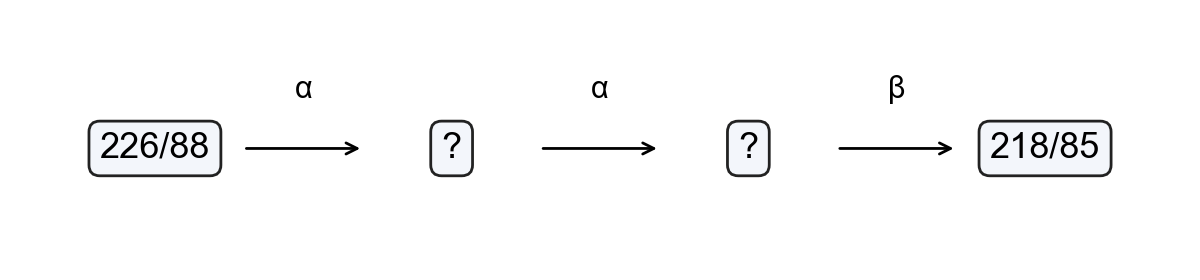
\includegraphics[width=0.86\linewidth]{rasmlar/gen/dc_297842.png}\end{center}
Oxirgi yadroning massa \textbf{sonini aniqlang.}

\noindent A)~\textsl{222} \hfill B)~\textsl{214} \hfill C)~\textsl{219} \hfill D)~\textsl{218}\par
\qsep
\noindent\qn{5.} Tarkibida 30\% SO\textsubscript{3} bo`lgan 100 g oleum 300 g suvga qo`shildi. Hosil bo`lgan eritmadagi H\textsubscript{2}SO\textsubscript{4} ning massa \textbf{ulushini (\%) aniqlang.}

\noindent A)~\textsl{17,5} \hfill B)~\textsl{26,69} \hfill C)~\textsl{35,58} \hfill D)~\textsl{40,03}\par
\qsep
\noindent\qn{6.} N\textsubscript{2} + 3H\textsubscript{2} $\rightleftarrows$ 2NH\textsubscript{3} reaksiyada muvozanat holatida [N\textsubscript{2}] = 1, [H\textsubscript{2}] = 0,5, [NH\textsubscript{3}] = 2 mol/l. Muvozanat \textbf{konstantasini (K) hisoblang.}

\noindent A)~\textsl{64} \hfill B)~\textsl{16} \hfill C)~\textsl{32} \hfill D)~\textsl{4}\par
\qsep
\noindent\qn{7.} 3 mol Al\textsubscript{2}(SO\textsubscript{4})\textsubscript{3} va 3 mol AlCl\textsubscript{3} suvda eritilib, eritma hajmi 2 l ga yetkazildi. Eritmadagi barcha ionlarning umumiy molyar \textbf{konsentratsiyasini (mol/l) aniqlang} (kuchli elektrolitlar to`liq dissotsilanadi).

\noindent A)~\textsl{3} \hfill B)~\textsl{27} \hfill C)~\textsl{13,5} \hfill D)~\textsl{6,75}\par
\qsep
\noindent\qn{8.} Jadvalda metall plastinkalarning tuz eritmalariga tushirilishidagi kuzatuvlar berilgan (``+'' -- metall ajraladi, reaksiya boradi; ``$-$'' -- reaksiya bormaydi):
\begin{center}
\renewcommand{\arraystretch}{1.15}
\fitbox{\begin{tabular}{|c|c|c|c|}\hline
\textbf{Metall} & \textbf{ZnSO\textsubscript{4} eritmasi} & \textbf{AgNO\textsubscript{3} eritmasi} & \textbf{CuSO\textsubscript{4} eritmasi} \\ \hline
Mg & + & + & + \\ \hline
Cu & $-$ & + & $-$ \\ \hline
Zn & $-$ & + & + \\ \hline
\end{tabular}}
\end{center}
Ushbu metallardan qaysi biri eng faol?

\noindent A)~\textsl{Cu} \hfill B)~\textsl{Mg} \hfill C)~\textsl{Zn} \hfill D)~\textsl{Fe}\par
\qsep
\noindent\qn{9.} 10 l H\textsubscript{2}S va 45 l O\textsubscript{2} aralashmasi 2H\textsubscript{2}S + 3O\textsubscript{2} $\to$ 2SO\textsubscript{2} + 2H\textsubscript{2}O tenglama bo`yicha to`liq reaksiyaga kirishdi (reaksiyadan so`ng suv suyuq holatda; gazlar bir xil sharoitda o`lchandi). Aralashma hajmi necha litrga o`zgargan (modul bo`yicha)?

\noindent A)~\textsl{55} \hfill B)~\textsl{40} \hfill C)~\textsl{10} \hfill D)~\textsl{15}\par
\qsep
\noindent\qn{10.} 8 g metall kislotada eritilganda 4,48 l (n.sh.) vodorod ajraldi. Metallning ekvivalent \textbf{massasini (g/mol) aniqlang} (\textit{V}\_E(H\textsubscript{2}) = 11,2 l/mol).

\noindent A)~\textsl{40} \hfill B)~\textsl{10} \hfill C)~\textsl{89,6} \hfill D)~\textsl{20}\par
\qsep
\noindent\qn{11.} Azot (\textit{Z} = 7) atomida nechta juftlashmagan elektron bor?

\noindent A)~\textsl{4} \hfill B)~\textsl{2} \hfill C)~\textsl{5} \hfill D)~\textsl{3}\par
\qsep
\noindent\qn{12.} Zichligi 1,4 g/ml bo`lgan 40\% li KOH eritmasining molyar \textbf{konsentratsiyasini (mol/l) aniqlang.}

\noindent A)~\textsl{1} \hfill B)~\textsl{20} \hfill C)~\textsl{10} \hfill D)~\textsl{7,14}\par
\qsep
\noindent\qn{13.} 61,25 g KClO\textsubscript{3} reaksiyaga kirishdi (2KClO\textsubscript{3} $\to$ 2KCl + 3O\textsubscript{2}). Ajralgan O\textsubscript{2} \textbf{hajmini (l, n.sh.) hisoblang} (unum 80\%).

\noindent A)~\textsl{13,44} \hfill B)~\textsl{16,8} \hfill C)~\textsl{26,88} \hfill D)~\textsl{6,72}\par
\qsep
\noindent\qn{14.} Ishqoriy metallar haqida qaysi fikrlar to`g`ri? 1) Ishqoriy metallar tabiatda erkin holda uchraydi; 2) Natriy yonganda Na\textsubscript{2}O\textsubscript{2} hosil bo`ladi; 3) Natriy kerosin ostida saqlanadi; 4) Litiy eng yengil metall

\noindent A)~\textsl{1, 2, 3} \hfill B)~\textsl{1, 4} \hfill C)~\textsl{2, 3, 4} \hfill D)~\textsl{1, 3}\par
\qsep
\noindent\qn{15.} Ca + 2H\textsubscript{2}O $\to$ Ca(OH)\textsubscript{2} + H\textsubscript{2} reaksiyasida 20 g Ca ishtirok etdi. H\textsubscript{2} \textbf{massasini (g) toping.}

\noindent A)~\textsl{1} \hfill B)~\textsl{2} \hfill C)~\textsl{0,5} \hfill D)~\textsl{1,5}\par
\qsep
\noindent\qn{16.} 11,2 g temir bir qismi xlor bilan, xuddi shuncha qismi xlorid kislota bilan reaksiyaga kirishdi. Hosil bo`lgan tuzlar massalari \textbf{farqini (g) aniqlang.}

\noindent A)~\textsl{32,5} \hfill B)~\textsl{25,4} \hfill C)~\textsl{14,2} \hfill D)~\textsl{7,1}\par
\qsep
\noindent\qn{17.} Reaksiya tenglamasi: Mg(HCO\textsubscript{3})\textsubscript{2} $\to$ MgCO\textsubscript{3} + CO\textsubscript{2} + H\textsubscript{2}O. Reaksiyaga 58,4 g Mg(HCO\textsubscript{3})\textsubscript{2} kirishdi (unum 50\%). CO\textsubscript{2} \textbf{miqdorini (mol) hisoblang.}

\noindent A)~\textsl{0,2} \hfill B)~\textsl{0,4} \hfill C)~\textsl{0,1} \hfill D)~\textsl{0,3}\par
\qsep
\noindent\qn{18.} Qaysi juftliklar o`zaro reaksiyaga kirishmaydi? 1) Fe\textsubscript{2}O\textsubscript{3} va H\textsubscript{2}O; 2) SiO\textsubscript{2} va H\textsubscript{2}O; 3) CO\textsubscript{2} va CaO; 4) ZnO va HCl

\noindent A)~\textsl{4} \hfill B)~\textsl{1, 2} \hfill C)~\textsl{1} \hfill D)~\textsl{2, 3, 4}\par
\qsep
\noindent\qn{19.} Reaksiya tenglamasi: 2Al + 3CuCl\textsubscript{2} $\to$ 2AlCl\textsubscript{3} + 3Cu. Reaksiyaga 27 g CuCl\textsubscript{2} kirishdi. Al \textbf{massasini (g) hisoblang.}

\noindent A)~\textsl{8,1} \hfill B)~\textsl{3,6} \hfill C)~\textsl{7,2} \hfill D)~\textsl{1,8}\par
\qsep
\noindent\qn{20.} C\textsubscript{4}H\textsubscript{9}OH tarkibli spirtlarning izomerlari soni nechta?

\noindent A)~\textsl{5} \hfill B)~\textsl{4} \hfill C)~\textsl{3} \hfill D)~\textsl{6}\par
\qsep
\noindent\qn{21.} 23 g etil spirtidan 90\% unum bilan etilen olindi. Etilen \textbf{hajmini (l, n.sh.) aniqlang.}

\noindent A)~\textsl{10,08} \hfill B)~\textsl{11,2} \hfill C)~\textsl{20,16} \hfill D)~\textsl{20,7}\par
\qsep
\noindent\qn{22.} Arenlar, neft va tabiiy gaz haqida qaysi fikrlar to`g`ri? 1) Benzolda 6 ta sp\textsuperscript{2} gibridlangan uglerod bor; 2) Benzol uchun birikish reaksiyalari mutlaqo xos emas; 3) Benzoldan nitrobenzol nitrolash bilan olinadi; 4) Naftalin -- bir halqali aren

\noindent A)~\textsl{1, 3, 4} \hfill B)~\textsl{1, 3} \hfill C)~\textsl{1, 4} \hfill D)~\textsl{1}\par
\qsep
\noindent\qn{23.} Spirt va fenollar haqida qaysi fikrlar to`g`ri? 1) Fenol Cu(OH)\textsubscript{2} ni eritib ko`k kompleks hosil qiladi; 2) Etanol natriy bilan reaksiyaga kirishadi; 3) Etilenglikol zaharsiz; 4) Birlamchi spirt oksidlanganda aldegid hosil bo`ladi

\noindent A)~\textsl{1, 2, 3} \hfill B)~\textsl{1, 2, 4} \hfill C)~\textsl{2, 4} \hfill D)~\textsl{1, 4}\par
\qsep
\noindent\qn{24.} Reaksiya tenglamasi: HCHO + Ag\textsubscript{2}O $\to$ HCOOH + 2Ag. Reaksiyaga 2,24 l (n.sh.) HCHO kirishdi. Ag\textsubscript{2}O \textbf{massasini (g) hisoblang.}

\noindent A)~\textsl{46,4} \hfill B)~\textsl{23,2} \hfill C)~\textsl{11,6} \hfill D)~\textsl{34,8}\par
\qsep
\noindent\qn{25.} 60 g CH\textsubscript{3}COOH dan quyidagi ikki bosqichda CH\textsubscript{4} olinadi: 1) CH\textsubscript{3}COOH + NaOH $\to$ CH\textsubscript{3}COONa + H\textsubscript{2}O (unum 50\%); 2) CH\textsubscript{3}COONa + NaOH $\to$ CH\textsubscript{4} + Na\textsubscript{2}CO\textsubscript{3} (unum 75\%). Oxirgi mahsulot CH\textsubscript{4} ning \textbf{hajmini (l, n.sh.) toping.}

\noindent A)~\textsl{16,8} \hfill B)~\textsl{11,2} \hfill C)~\textsl{8,4} \hfill D)~\textsl{22,4}\par
\qsep
\noindent\qn{26.} 445 g tristearin natriy ishqori bilan to`liq gidrolizlanganda necha gramm sovun hosil bo`ladi?

\noindent A)~\textsl{153} \hfill B)~\textsl{306} \hfill C)~\textsl{459} \hfill D)~\textsl{445}\par
\qsep
\noindent\qn{27.} 22 g CO\textsubscript{2} dan quyidagi ikki bosqichda C\textsubscript{2}H\textsubscript{5}OH olinadi: 1) 6CO\textsubscript{2} + 6H\textsubscript{2}O $\to$ C\textsubscript{6}H\textsubscript{12}O\textsubscript{6} + 6O\textsubscript{2} (unum 60\%); 2) C\textsubscript{6}H\textsubscript{12}O\textsubscript{6} $\to$ 2C\textsubscript{2}H\textsubscript{5}OH + 2CO\textsubscript{2} (unum 90\%). Oxirgi mahsulot C\textsubscript{2}H\textsubscript{5}OH ning \textbf{massasini (g) toping.}

\noindent A)~\textsl{4,14} \hfill B)~\textsl{6,9} \hfill C)~\textsl{4,6} \hfill D)~\textsl{7,67}\par
\qsep
\noindent\qn{28.} 24,6 g C\textsubscript{6}H\textsubscript{5}NO\textsubscript{2} dan quyidagi ikki bosqichda C\textsubscript{6}H\textsubscript{5}NH\textsubscript{3}Cl olinadi: 1) C\textsubscript{6}H\textsubscript{5}NO\textsubscript{2} + 3H\textsubscript{2} $\to$ C\textsubscript{6}H\textsubscript{5}NH\textsubscript{2} + 2H\textsubscript{2}O (unum 80\%); 2) C\textsubscript{6}H\textsubscript{5}NH\textsubscript{2} + HCl $\to$ C\textsubscript{6}H\textsubscript{5}NH\textsubscript{3}Cl (unum 75\%). Oxirgi mahsulot C\textsubscript{6}H\textsubscript{5}NH\textsubscript{3}Cl ning \textbf{massasini (g) toping.}

\noindent A)~\textsl{15,54} \hfill B)~\textsl{19,42} \hfill C)~\textsl{20,72} \hfill D)~\textsl{25,9}\par
\qsep
\noindent\qn{29.} 3C\textsubscript{2}H\textsubscript{2} (C, t) reaksiyasi natijasida qaysi organik modda hosil bo`ladi?

\noindent\begin{tabular}{@{}p{0.47\linewidth}@{}p{0.47\linewidth}@{}}
A)~\textsl{benzoy kislota} & B)~\textsl{etilatsetat} \\
C)~\textsl{benzol} & D)~\textsl{sirka aldegid} \\
\end{tabular}\par
\qsep
\noindent\qn{30.} Uch probirkada (\textit{X}, \textit{Y}, \textit{Z}) Na\textsubscript{2}SO\textsubscript{4}, K\textsubscript{2}CO\textsubscript{3}, NH\textsubscript{4}Cl eritmalari bor (tartibsiz). Ularga HCl va NaOH ta'sir ettirildi. Kuzatuvlar jadvalda:
\begin{center}
\renewcommand{\arraystretch}{1.15}
\fitbox{\begin{tabular}{|c|c|c|}\hline
\textbf{Probirka} & \textbf{HCl qo`shilganda} & \textbf{NaOH qo`shib qizdirilganda} \\ \hline
\textit{X} & o`zgarish yo`q & o`tkir hidli gaz ajraladi \\ \hline
\textit{Y} & o`zgarish yo`q & o`zgarish yo`q \\ \hline
\textit{Z} & gaz ajraladi & o`zgarish yo`q \\ \hline
\end{tabular}}
\end{center}
\textit{X}, \textit{Y}, \textit{Z} probirkalardagi \textbf{moddalarni aniqlang.}
\noindent A)~\textsl{\textit{X} -- K\textsubscript{2}CO\textsubscript{3}, \textit{Y} -- NH\textsubscript{4}Cl, \textit{Z} -- Na\textsubscript{2}SO\textsubscript{4}}\par
\noindent B)~\textsl{\textit{X} -- NH\textsubscript{4}Cl, \textit{Y} -- K\textsubscript{2}CO\textsubscript{3}, \textit{Z} -- Na\textsubscript{2}SO\textsubscript{4}}\par
\noindent C)~\textsl{\textit{X} -- Na\textsubscript{2}SO\textsubscript{4}, \textit{Y} -- NH\textsubscript{4}Cl, \textit{Z} -- K\textsubscript{2}CO\textsubscript{3}}\par
\noindent D)~\textsl{\textit{X} -- NH\textsubscript{4}Cl, \textit{Y} -- Na\textsubscript{2}SO\textsubscript{4}, \textit{Z} -- K\textsubscript{2}CO\textsubscript{3}}\par
\qsep
\noindent\qn{31.} Rasmda spirt lampasining tuzilishi ko`rsatilgan. 1 raqami bilan \textbf{belgilang}an qism nima deb ataladi?
\begin{center}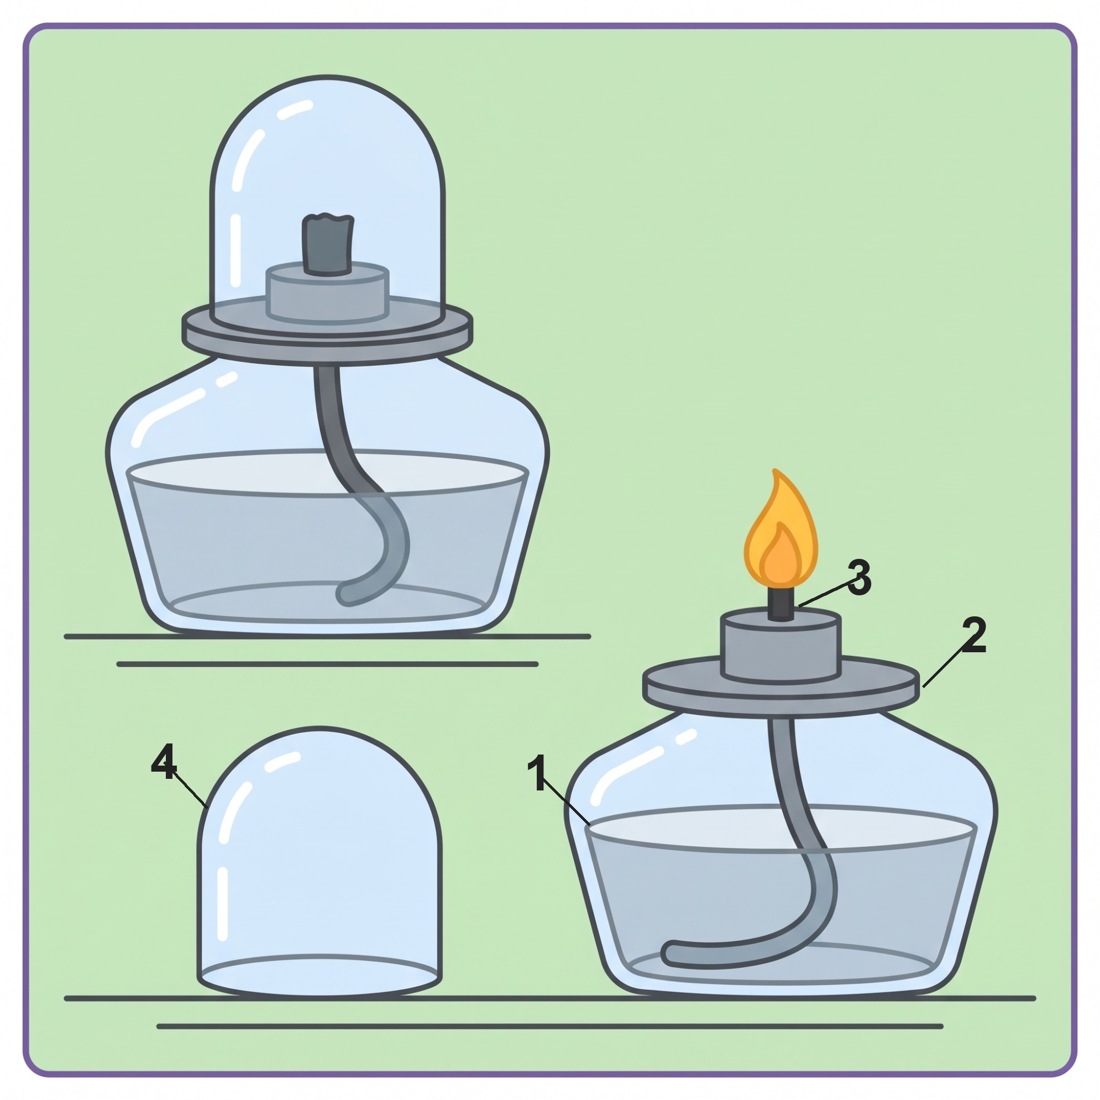
\includegraphics[width=0.86\linewidth]{rasmlar/darslik/d_spirt_lampa.png}\end{center}

\noindent A)~\textsl{idish} \hfill B)~\textsl{tutqich} \hfill C)~\textsl{pilik} \hfill D)~\textsl{shtativ}\par
\qsep
\noindent\qn{32.} 300 g 10\% li va 100 g 40\% li KCl eritmalari aralashtirildi. Yangi eritmaning massa \textbf{ulushini (\%) toping.}

\noindent\begin{tabular}{@{}p{0.47\linewidth}@{}p{0.47\linewidth}@{}}
A)~\textsl{25} & B)~\textsl{50} \\
C)~\textsl{15,75} & D)~\textsl{17,5   ---} \\
\end{tabular}\par
\qsep
\end{multicols}
\medskip
\noindent\setlength{\fboxsep}{0pt}\fbox{\begin{tabular}{p{0.74\linewidth}|p{0.2\linewidth}}
\parbox[t]{0.72\linewidth}{\vspace{3pt}\textbf{Topshiriqlar (33--35) va javob variant (A--F)larini o`zaro to`g`ri moslashtiring.} KI va NaBr dan iborat 18,6 g aralashma suvda eritilib, mo`l AgNO\textsubscript{3} eritmasi qo`shildi; hosil bo`lgan cho`kmalarning umumiy massasi 30,55 g.
\vspace{3pt}} & \parbox[t]{0.19\linewidth}{\vspace{3pt}A~\textsl{8,3}\\[3pt]
B~\textsl{204}\\[3pt]
C~\textsl{13,55}\\[3pt]
D~\textsl{510}\\[3pt]
E~\textsl{6,64}\\[3pt]
F~\textsl{255}}\\ \hline
\parbox[t]{0.72\linewidth}{\vspace{2pt}\textbf{33. Aralashmadagi KI massasini (g) aniqlang.}\vspace{2pt}} & \\ \hline
\parbox[t]{0.72\linewidth}{\vspace{2pt}\textbf{34. Sarflangan 10\% li AgNO\textsubscript{3} eritmasining massasini (g) aniqlang (M(AgNO\textsubscript{3}) = 170 g/mol).}\vspace{2pt}} & \\ \hline
\parbox[t]{0.72\linewidth}{\vspace{2pt}\textbf{35. Eritmada hosil bo`lgan nitratlarning umumiy massasini (g) aniqlang.}\vspace{2pt}} & 
\end{tabular}}
\par\bigskip
\noindent\qn{36.} KMnO\textsubscript{4} + FeSO\textsubscript{4} + H\textsubscript{2}SO\textsubscript{4} $\to$ MnSO\textsubscript{4} + Fe\textsubscript{2}(SO\textsubscript{4})\textsubscript{3} + K\textsubscript{2}SO\textsubscript{4} + H\textsubscript{2}O reaksiya tenglamasini tenglang va barcha koeffitsiyentlar \textbf{yig`indisini aniqlang.}
\javob\qsep
\noindent\qn{37.} Ketma-ket ulangan ikkita elektrolizyordan (CuSO\textsubscript{4} va AgNO\textsubscript{3} eritmalari, inert elektrodlar) tok o`tkazildi. Birinchi elektrolizyor katodida 12,8 g mis ajraldi. Ikkala elektrolizyor anodlarida ajralgan kislorodning umumiy \textbf{hajmini (l, n.sh.) toping} (anodda ikkalasida ham O\textsubscript{2} ajraladi).
\javob\qsep
\noindent\qn{38.} Alyuminiy (0,1 mol) va rux (0,1 mol) aralashmasi mo`l xlorid kislotada eritildi. Ajralgan vodorodning \textbf{hajmini (l, n.sh.) aniqlang.}
\javob\qsep
\noindent\qn{39.} 90 g glyukoza spirtli bijg`ish natijasida etanolga (unum 80\%), hosil bo`lgan etanol esa sirka kislotagacha (unum 80\%) aylantirildi. Olingan kislotani to`liq neytrallash uchun NaOH ning \textbf{massasini (g) toping.}
\javob\qsep
\noindent\qn{40.} 162 g kraxmal to`liq gidrolizlanib (unum 100\%), hosil bo`lgan glyukoza \textbf{massasini (g) aniqlang.}
\javob\qsep
\par\bigskip\begin{center}\textbf{\fontsize{13}{15}\selectfont YOZMA ISH}\end{center}
\noindent\qn{41.} \textbf{Topshiriqni bajarish jarayonida barcha reaksiya tenglamalarini yozing. Miqdoriy va arifmetik hisoblashlarni (unga asos bo`lgan usul yoki formulani ko`rsatgan holda) uzviy ketma-ketlikda bajaring.}\par\smallskip
CuSO\textsubscript{4}$\cdot$5H\textsubscript{2}O va Na\textsubscript{2}SO\textsubscript{4}$\cdot$10H\textsubscript{2}O dan iborat 114,4 g aralashma 300 g suvda eritildi. Eritma inert elektrodlar yordamida 5 A tok kuchi bilan 7720 s elektroliz qilindi; shu vaqt tugaganda eritmadagi Cu\textsuperscript{2+} ionlari to`liq tugagan edi.\par
\noindent 1)Aralashmadagi kristallogidratlarning massalarini (g) aniqlang.\par
\noindent 2)Dastlabki eritmada CuSO\textsubscript{4} va Na\textsubscript{2}SO\textsubscript{4} ning massa ulushlarini (\%) toping. Elektroliz davomida o`tgan zaryadni (C) ham hisoblang.\par
\noindent 3)Anodda ajralgan gazning hajmini (l, n.sh.) va elektroliz tugagandan keyingi eritma massasini (g) aniqlang.\par
\noindent 4)Elektroliz tugagach eritmadagi H\textsubscript{2}SO\textsubscript{4} va Na\textsubscript{2}SO\textsubscript{4} ning massa ulushlarini (\%) hisoblang. Dastlabki CuSO\textsubscript{4} ning massasini (g) ham hisoblang.\par
\noindent 5)Shu eritmani to`liq neytrallash uchun zichligi 1,22 g/ml bo`lgan 20\% li NaOH eritmasidan necha ml kerak? Agar tok kuchi 2 marta oshirilsa, xuddi shu miqdor Cu ajralishi uchun necha sekund kerak bo`ladi?\par
\diqqat{Mazkur topshiriq kengaytirilgan javobni talab etib, uning yechilish usuli va shu usul asosidagi barcha hisoblash amallari javoblar varaqasida aks etishi lozim.}\qsep
\noindent\qn{42.} Quyidagi o`zgarishlar zanjirida \textit{X}, \textit{Y}, \textit{Z} noma'lum organik moddalar:\par
\[\setlength{\fboxsep}{0pt}\text{CH\textsubscript{3}Cl}\xrightarrow{\text{Na}}\text{\textit{X}}\xrightarrow{\text{Cl\textsubscript{2}, yorug`lik}}\text{\textit{Y}}\xrightarrow{\text{KOH (suvli)}}\text{C\textsubscript{2}H\textsubscript{5}OH}\]
\noindent 1)CH\textsubscript{3}Cl $\to$ \textit{X} : reaksiya tenglamasini yozing; hosil bo`lgan moddani nomlang.\par
\noindent 2)\textit{X} $\to$ \textit{Y} : reaksiya tenglamasini yozing; hosil bo`lgan moddani nomlang.\par
\noindent 3)\textit{Y} $\to$ C\textsubscript{2}H\textsubscript{5}OH : reaksiya tenglamasini yozing; hosil bo`lgan moddani nomlang.\par
\diqqat{Mazkur topshiriq kengaytirilgan javobni talab etib, uning yechilish usuli va shu usul asosidagi barcha hisoblash amallari javoblar varaqasida aks etishi lozim.}\qsep
\noindent\qn{43.} \textbf{Topshiriqni bajarish jarayonida barcha reaksiya tenglamalarini yozing. Miqdoriy va arifmetik hisoblashlarni (unga asos bo`lgan usul yoki formulani ko`rsatgan holda) uzviy ketma-ketlikda bajaring.}\par\smallskip
50 m\textsuperscript{3} qattiq suvda Ca(HCO\textsubscript{3})\textsubscript{2} ning konsentratsiyasi 40 mol/m\textsuperscript{3}, Mg(HCO\textsubscript{3})\textsubscript{2} niki 10 mol/m\textsuperscript{3} ga teng (1 m\textsuperscript{3} = 1000 l).\par
\noindent 1)Suv qaynatilganda qanday reaksiyalar sodir bo`lishini yozing.\par
\noindent 2)Qaynatish natijasida hosil bo`ladigan CaCO\textsubscript{3} cho`kmasi massasini (kg) hisoblang. Qaynatish bilan ajralgan CO\textsubscript{2} hajmini (m\textsuperscript{3}, n.sh.) ham hisoblang.\par
\noindent 3)Mg(HCO\textsubscript{3})\textsubscript{2} dan hosil bo`ladigan MgCO\textsubscript{3} massasini (kg) toping.\par
\noindent 4)Suvni yumshatish uchun sodadan (Na\textsubscript{2}CO\textsubscript{3}) necha kilogramm kerakligini hisoblang (Ca\textsuperscript{2+} va Mg\textsuperscript{2+} ni to`liq cho`ktirish uchun).\par
\noindent 5)Suvni ohak sutini (Ca(OH)\textsubscript{2}) bilan yumshatishda zarur Ca(OH)\textsubscript{2} massasini (kg) hisoblang (Ca(HCO\textsubscript{3})\textsubscript{2} + Ca(OH)\textsubscript{2} $\to$ 2CaCO\textsubscript{3} + 2H\textsubscript{2}O; Mg(HCO\textsubscript{3})\textsubscript{2} + 2Ca(OH)\textsubscript{2} $\to$ Mg(OH)\textsubscript{2} + 2CaCO\textsubscript{3} + 2H\textsubscript{2}O).\par
\diqqat{Mazkur topshiriq kengaytirilgan javobni talab etib, uning yechilish usuli va shu usul asosidagi barcha hisoblash amallari javoblar varaqasida aks etishi lozim.}\qsep
\newpage
\noindent\textbf{\fontsize{13}{15}\selectfont Nazorat testi}\ \textit{$\cdot$ 2-variant}\hfill \textbf{Javoblar kaliti}\par\smallskip\hrule\smallskip
\textit{Faqat o`qituvchi uchun.}\par\medskip
\noindent\textbf{1--32-savollar}\par\smallskip
\noindent\begin{tabular}{|c|c|c|c|c|c|c|c|c|c|c|c|c|c|c|c|}\hline
\textbf{1} & \textbf{2} & \textbf{3} & \textbf{4} & \textbf{5} & \textbf{6} & \textbf{7} & \textbf{8} & \textbf{9} & \textbf{10} & \textbf{11} & \textbf{12} & \textbf{13} & \textbf{14} & \textbf{15} & \textbf{16}\\\hline
\textsl{A} & \textsl{B} & \textsl{D} & \textsl{D} & \textsl{B} & \textsl{C} & \textsl{C} & \textsl{B} & \textsl{D} & \textsl{D} & \textsl{D} & \textsl{C} & \textsl{A} & \textsl{C} & \textsl{A} & \textsl{D}\\\hline
\textbf{17} & \textbf{18} & \textbf{19} & \textbf{20} & \textbf{21} & \textbf{22} & \textbf{23} & \textbf{24} & \textbf{25} & \textbf{26} & \textbf{27} & \textbf{28} & \textbf{29} & \textbf{30} & \textbf{31} & \textbf{32}\\\hline
\textsl{A} & \textsl{B} & \textsl{B} & \textsl{B} & \textsl{A} & \textsl{B} & \textsl{C} & \textsl{B} & \textsl{C} & \textsl{C} & \textsl{A} & \textsl{A} & \textsl{C} & \textsl{D} & \textsl{A} & \textsl{D}\\\hline
\end{tabular}\par\medskip
\noindent\textbf{33--35-savollar}\par\smallskip
\noindent\begin{tabular}{|c|c|c|}\hline \textbf{No} & \textbf{Javob} & \textbf{Qiymat}\\\hline
33 & \textsl{A} & 8,3\\\hline
34 & \textsl{F} & 255\\\hline
35 & \textsl{C} & 13,55\\\hline
\end{tabular}\par\medskip
\noindent\textbf{36--40-savollar}\par\smallskip
\noindent\begin{tabular}{|c|c|}\hline \textbf{No} & \textbf{To`g`ri javob}\\\hline
36 & 36\\\hline
37 & 4,48\\\hline
38 & 5,6\\\hline
39 & 25,6\\\hline
40 & 180\\\hline
\end{tabular}\par\medskip
\noindent\textbf{41--43-topshiriqlar: javoblar}\par\smallskip
\noindent\textbf{41-topshiriq.}\par
\noindent 1) 50 g; 64,4 g\par
\noindent 2) 7,72\%; 6,85\%; 38600 C\par
\noindent 3) 2,24 l; 398,4 g\par
\noindent 4) 4,92\%; 7,13\%; 32 g\par
\noindent 5) 65,6 ml; 3860 s\par
\noindent\textbf{42-topshiriq.}\par
\noindent 1) CH\textsubscript{3}Cl + Na $\to$ C\textsubscript{2}H\textsubscript{6} (etan)\par
\noindent 2) C\textsubscript{2}H\textsubscript{6} + Cl\textsubscript{2}, yorug`lik $\to$ C\textsubscript{2}H\textsubscript{5}Cl (xloretan)\par
\noindent 3) C\textsubscript{2}H\textsubscript{5}Cl + KOH (suvli) $\to$ C\textsubscript{2}H\textsubscript{5}OH (etanol)\par
\noindent\textbf{43-topshiriq.}\par
\noindent 1) Ca(HCO\textsubscript{3})\textsubscript{2} $\to$ CaCO\textsubscript{3}$\downarrow$ + CO\textsubscript{2}$\uparrow$ + H\textsubscript{2}O; Mg(HCO\textsubscript{3})\textsubscript{2} $\to$ MgCO\textsubscript{3}$\downarrow$ + CO\textsubscript{2}$\uparrow$ + H\textsubscript{2}O\par
\noindent 2) 200 kg; 56 m\textsuperscript{3}\par
\noindent 3) 42 kg\par
\noindent 4) 265 kg\par
\noindent 5) 222 kg\par
\par\bigskip\noindent\textbf{Mavzular taqsimoti}\par\smallskip
{\small\noindent\begin{longtable}{|c|p{7.2cm}|p{5.4cm}|c|}\hline \textbf{No} & \textbf{Mavzu} & \textbf{Tekshiriladigan ko`nikma} & \textbf{Ball}\\\hline
1 & Tirkashev III bob (eritmalar, jadval) & Jadval tahlili & 1\\\hline
2 & 7-sinf; Tirkashev (kristallogidrat) & Hisoblash va masala yechish & 1\\\hline
3 & 8-sinf (davriy qonun, diagramma) & Grafik tahlili & 1\\\hline
4 & 11-sinf (yadro reaksiyalari) & Rasm bo`yicha tahlil & 1\\\hline
5 & Tirkashev III bob (oleum); Tashev & Hisoblash va masala yechish & 1\\\hline
6 & Tirkashev VI bob (kimyoviy muvozanat) & Hisoblash va masala yechish & 1\\\hline
7 & Tirkashev IV bob (kuchli elektrolitlar) & Hisoblash va masala yechish & 1\\\hline
8 & Tirkashev \textit{V} bob (kuchlanish qatori, jadval) & Jadval tahlili & 1\\\hline
9 & 8-sinf (Gey-Lyussak qonuni) & Hisoblash va masala yechish & 1\\\hline
10 & 11-sinf (ekvivalentlar qonuni) & Hisoblash va masala yechish & 1\\\hline
11 & Tirkashev I bob; 8-sinf (elektron konfiguratsiya) & Bilim va tushunish & 1\\\hline
12 & 11-sinf 4-bob (molyar konsentratsiya) & Hisoblash va masala yechish & 1\\\hline
13 & 8-sinf; 9-sinf (stexiometriya) & Hisoblash va masala yechish & 1\\\hline
14 & 9-sinf (ishqoriy metallar); Tashev & Bilim va tushunish & 1\\\hline
15 & 9-sinf; Tirkashev (IIA/IIIA metallar (Ca,Mg,Al), hisob) & Hisoblash va masala yechish & 1\\\hline
16 & 9-sinf; Tashev (temir) & Hisoblash va masala yechish & 1\\\hline
17 & 9-sinf; Tirkashev (suv qattiqligi, hisob) & Hisoblash va masala yechish & 1\\\hline
18 & 9-sinf; Tashev (anorganik birikmalar xossalari) & Bilim va tushunish & 1\\\hline
19 & 9-sinf; Tirkashev (genetik zanjir/reaksiya turlari, hisob) & Hisoblash va masala yechish & 1\\\hline
20 & 10-sinf \S{}6, \S{}12, \S{}20, \S{}28 (izomeriya) & Bilim va tushunish & 1\\\hline
21 & 10-sinf \S{}21 (etilen olinishi) & Hisoblash va masala yechish & 1\\\hline
22 & 10-sinf (mavzuga oid paragraflar); Abdusamatov & Bilim va tushunish & 1\\\hline
23 & 10-sinf (mavzuga oid paragraflar); Abdusamatov & Bilim va tushunish & 1\\\hline
24 & 10-sinf (ald, hisob) & Hisoblash va masala yechish & 1\\\hline
25 & 10-sinf (ikki bosqichli hisob) & Hisoblash va masala yechish & 1\\\hline
26 & 10-sinf \S{}29 (yog`lar, sovunlanish) & Hisoblash va masala yechish & 1\\\hline
27 & 10-sinf (ikki bosqichli hisob) & Hisoblash va masala yechish & 1\\\hline
28 & 10-sinf (ikki bosqichli hisob) & Hisoblash va masala yechish & 1\\\hline
29 & 10-sinf (olinish usullari) & Bilim va tushunish & 1\\\hline
30 & 7--10-sinf va Tashev (laboratoriya ishlari, sifat reaksiyalar) & Jadval tahlili & 1\\\hline
31 & 7-sinf (laboratoriya jihozlari, 3-rasm) & Rasm bo`yicha tahlil & 1\\\hline
32 & Tirkashev III bob (eritmalar) & Hisoblash va masala yechish & 1\\\hline
33--35 & Aralash masala (moslashtirish) & Ko`p bosqichli hisob & 3\\\hline
36--40 & Qisqa javobli masalalar & Hisoblash & 5\\\hline
41--43 & Yozma ish & Usul va hisob (M, A) & 75\\\hline
\end{longtable}}
\end{document}
